\documentclass[10pt,aspectratio=1610]{beamer} % use option aspectratio=169 or 1610 for wide slides
% Note: For online presentations via Zoom use the ratio of the screen you want to share
\usetheme{Rochester}

% load syscop style
\usepackage{style/syscop}

%--------------------------------------------------
% TITLE
%--------------------------------------------------

% NOTE: what's in [ ] goes to footer for the fields title, author and date
\title[Regularization techniques for a Riccati-based Interior-Point QP Solver]{\huge Regularization techniques for a Riccati-based Interior-Point QP Solver}
\author[J. Xiong, J. Frey, K. Baumgärtner and M. Diehl]{Jingtao Xiong, Jonathan Frey, Katrin Baumgärtner and Moritz Diehl}
\institute{Systems Control and Optimization Laboratory (syscop)}
\date[\today]{Group Retreat \\ \today }


%--------------------------------------------------
% Useful packages
%--------------------------------------------------

\usepackage{mathtools}
\usepackage{mathdots}
\usepackage{graphicx}
\usepackage{optidef}
\usepackage{booktabs}
\usepackage{diagbox}
\usepackage{multirow}
\usepackage{geometry}
\usepackage{subcaption}
\usepackage{nicematrix}

\begin{document}

\InsertTitle

\begin{frame}{Content}

	\begin{itemize}
		\item Riccati-based Interior-Point Method
		\item Regularization techniques
		\item Numerical experiments
		\item Conclusion
	\end{itemize}

\end{frame}

\begin{frame}{Riccati-based Interior-Point Method}
    \framesubtitle{QP formulation}
    Consider a QP with equality $Fy=b$ and inequality constraints $Gy \le d$, by introducing slacks $t$,
    we have following formulation:
    \begin{mini}
        {y, t}
        {\frac{1}{2} y^T H y + g^T y}
        {\label{eq:qp_problem}}
        {}
        \addConstraint{F y}{= b}
        \addConstraint{G y + t}{= d}
        \addConstraint{t}{\ge 0}
    \end{mini}
    \pause
    \vspace{0.5em}
    The corresponding IPM-KKT conditions are:
    \begin{equation}
        r(y, t, \pi, \lambda) =
        \begin{bmatrix}
            H y + g + F^T \pi + G^T \lambda \\
            F y - b \\
            G y + t - d \\
            T \Lambda \mathbf{1} - \sigma \mu \mathbf{1}
        \end{bmatrix} = 0
    \end{equation}
    where $T = \mathrm{diag}(t)$, $\Lambda = \mathrm{diag}(\lambda)$, $\pi$ and $\lambda$ are dual variables for equality and inequality constraints respectively,
    $\sigma$ is the centering parameter and $\mu$ is the duality measure.
\end{frame}

\begin{frame}{Riccati-based Interior-Point Method}
    \framesubtitle{Primal-Dual Interior-Point Method}
	At each iteration $i$, we solve the following linear system to get the descent direction:
	\begin{equation}
		\begin{bmatrix}
		H & F^T & G^T & 0\\
		F & 0 & 0 & 0 \\
		G & 0 & 0 & I \\
		0 & 0 & T_i & \Lambda_i
		\end{bmatrix}
		\begin{bmatrix}
		\Delta y \\
		\Delta \pi \\
        \Delta \lambda \\
		\Delta t
		\end{bmatrix} = -
		\begin{bmatrix}
            Hy_i + g + F^T \pi_i + G^T \lambda_i \\
            Fy_i - b \\
            Gy_i + t_i - d \\
            T_i \Lambda_i \mathbf{1} - \sigma_i \mu_i \mathbf{1}
        \end{bmatrix} = -
		\begin{bmatrix}
		r_{\mathrm{stat}}^i \\
		r_{\mathrm{eq}}^i \\
		r_{\mathrm{ineq}}^i \\
		r_{\mathrm{comp}}^i
		\end{bmatrix}
	\end{equation}
    \pause
	Eliminating $\Delta t$ and $\Delta \lambda$ based on Schur Complement, we obtain the following Reduced system:
	\begin{equation}
		\begin{bmatrix}
		 H + G^T \Lambda_i T_i^{-1} G & F^T \\
		F & 0
		\end{bmatrix}
		\begin{bmatrix}
		\Delta y \\
		\Delta \pi
		\end{bmatrix} = -
		\begin{bmatrix}
		r_{\mathrm{stat}}^i - G^T T_i^{-1} ( \Lambda_i r_{\mathrm{ineq}}^i - r_{\mathrm{comp}}^i ) \\
		r_{\mathrm{eq}}^i
		\end{bmatrix}
	\end{equation}
    where $G^T \Lambda_i T_i^{-1} G$ can be regarded as the curvature contribution from inequality constraints.\\
    \vspace{0.5em}
    We can define $\tilde{H} = H + G^T \Lambda_i T_i^{-1} G$ and $\tilde{r}_{\mathrm{stat}}^i = r_{\mathrm{stat}}^i - G^T T_i^{-1} ( \Lambda_i r_{\mathrm{ineq}}^i - r_{\mathrm{comp}}^i )$. for simplicity.
\end{frame}

\begin{frame}{Riccati-based Interior-Point Method}
    \framesubtitle{Riccati recursion for solving OCP structure QP}
    
    In Optimal Control Problems (OCP), We can interleave the Reduced system as follows:
    \begin{equation*}
        \begin{bNiceMatrix}[margin]
            \ddots & & & & \\
            & 0 & -I \\
            & -I & \tilde{Q}_k & \tilde{S}_k^T & A_k^T \\
            & 0 & \tilde{S}_k & \tilde{R}_k & B_k^T \\
            & 0 & A_k & B_k & 0 \\
            &  &  &  &  & \ddots
        \CodeAfter
            \SubMatrix({3-3}{4-4})
        \end{bNiceMatrix}
        \begin{bmatrix}
            \vdots \\
            \Delta \pi_k \\
            \Delta x_k \\
            \Delta u_k \\
            \Delta \pi_{k+1}\\
            \vdots
        \end{bmatrix} = -
        \begin{bmatrix}
            \vdots \\
            r_{\mathrm{eq}}^{k-1} \\
            \tilde{r}_{\mathrm{stat}, x}^k \\
            \tilde{r}_{\mathrm{stat}, u}^k \\
            r_{\mathrm{eq}}^k \\
            \vdots
        \end{bmatrix}
    \end{equation*}
    where $\tilde{H}_k$ can be decomposed into the state cost matrix $\tilde{Q}_k$, the control cost matrix $\tilde{R}_k$, and the cross-term cost matrix $\tilde{S}_k$ at stage $k$, and $A_k$, $B_k$ are dynamics matrices at stage $k$.
\end{frame}

\begin{frame}{Riccati-based Interior-Point Method}
    \framesubtitle{Riccati recursion for solving OCP structure QP}
    With OCP structure, the Reduced system can be solved in O(N) via Riccati recursion. The main steps are as follows:
    \pause
	\begin{itemize}
        \item \textbf{Backward recursion:} (For $k = N-1, \dots, 0$ with $P_N = \tilde{Q}_N, p_N = \tilde{r}_{\mathrm{stat}, x}^N$)
        \begin{equation*}
            \begin{aligned}
                \alert{M_k} & \alert{= \tilde{R}_k + B_k^T P_{k+1} B_k}, \quad W_k = \tilde{S}_k + B_k^T P_{k+1} A_k \\
                K_k &= -M_k^{-1} W_k \\
				\quad k_k &= -M_k^{-1} (\tilde{r}_{\mathrm{stat}, u}^k + B_k^T (P_{k+1} r_{\mathrm{eq}}^k + p_{k+1})) \\
                P_k &= \tilde{Q}_k + A_k^T P_{k+1} A_k - W_k^T M_k^{-1} W_k \\
                p_k &= \tilde{r}_{\mathrm{stat}, x}^k + A_k^T (P_{k+1} r_{\mathrm{eq}}^k + p_{k+1}) + W_k^T k_k
            \end{aligned}
	\end{equation*}
    \pause
		\item \textbf{Forward recursion:} (For $k = 0, \dots, N-1$)
        \begin{equation*}
            \begin{aligned}
                \Delta u_k &= K_k \Delta x_k + k_k \\
                \Delta x_{k+1} &= A_k \Delta x_k + B_k \Delta u_k + r_{\mathrm{eq}}^k \\
				\Delta t_k &= -(G_{x}^k \Delta x_k + G_{u}^k \Delta u_k + r_{\mathrm{ineq}}^k) \\
				\Delta \lambda_k &= T_k^{-1} (-r_{\mathrm{comp}}^k - \Lambda_k \Delta t_k)
            \end{aligned}
        \end{equation*}
	\end{itemize}
\end{frame}

\begin{frame}{Regularization techniques}
    \framesubtitle{Motivation for regularization}
	When the Hessian $H$ is indefinite (indefinite QP), regularization is introduced to recover positive definiteness and find a descent direction, 
    which can be applied to: 
    \pause
    \begin{itemize}
        \item Full Hessian $H_k$ at each stage
        \pause
        \item Reduced Hessian $M_k = R_k + B_k^T P_{k+1} B_k$ during Riccati recursions
    \end{itemize}
    \pause
    And the regularized Reduced KKT system can be written as:
	\begin{equation}
		\begin{bmatrix}
		 \tilde{H} + E & F^T \\
		F & 0
		\end{bmatrix}
		\begin{bmatrix}
		\Delta y \\
		\Delta \pi
		\end{bmatrix} = -
		\begin{bmatrix}
		\tilde{r}_{\mathrm{stat}}^i \\
		r_{\mathrm{eq}}^i
		\end{bmatrix}
	\end{equation}
    where $E$ is the regularization matrix, which can be designed in various ways while preserving the OCP structure, such as:
    \begin{itemize}
        \item Eigenvalue Modification (EM)
        \item Cholesky Modification (CM)
        \item Levenberg-Marquardt (LM)
    \end{itemize}
    \pause
    In this project, we mainly focus on the regularization based on Eigenvalue Modification (EM).
\end{frame}

\begin{frame}{Regularization techniques}
    \framesubtitle{Full Hessian regularization}
    To ensure the positive definiteness of $H_k$ at stage $k$, common methods include:
	\begin{itemize}
		\item PROJECT
		\begin{equation*}
		    \mathrm{project}(H_k, \epsilon) := V_k [\max(\epsilon, D_k)] V_k^{-1}
		\end{equation*}
		\item MIRROR
		\begin{equation*}
			\mathrm{mirror}(H_k, \epsilon) := V_k [\max(\epsilon, \mathrm{abs}(D_k))] V_k^{-1}
		\end{equation*}
	\end{itemize}
    where $H_k = V_k D_k V_k^{-1}$ is the eigenvalue decomposition of $H_k$, and $\epsilon > 0$ is a small positive constant. \\
    \begin{itemize}
        \item Pros:
            \begin{itemize}
                \item Minimum Frobenius norm change to $H_k$
                \item Sound and robust in practice
            \end{itemize}
        \item Cons:
            \begin{itemize}
                \item Ignore the possibility of utilizing the positive definiteness of Reduced Hessian $M_k$, which already ensures a descent direction in Reduced space
            \end{itemize}
    \end{itemize}
\end{frame}

\begin{frame}{Regularization techniques}
    \framesubtitle{Reduced Hessian regularization}
    Based on the drawback of Full Hessian regularization, we try to regularize only the Reduced Hessian $M_k$ during Riccati recursions.\\
    \vspace{0.5em}
    With $M_k = R_k + B_k^T P_{k+1} B_k$, we propose the following regularization techniques, when the Cholesky factorization fails at current stage:
    \pause
	\vspace{0.5em}
    \begin{itemize}
		\item M\_STAGE\_EM:
        \\ Directly regularize $M_k$ by eigenvalue modification
		\item PM\_STAGE\_EM:
        \\ Regularize $P_{k+1}$ by eigenvalue modification in $M_k$ first, then regularize P-modified $M_k$ by eigenvalue modification
		\item RP\_STAGE\_EM:
        \\ Regularize $R_k$ and $P_{k+1}$ by eigenvalue modification in $M_k$
	\end{itemize}
    \vspace{0.5em}
    All of them can have two variants, i.e. PROJECT and MIRROR versions.
\end{frame}

\begin{frame}{Numerical experiments}
    \framesubtitle{Prototype implementation}
    We implemented a prototype solver in Python, aiming to solve the following OCP structure QP:

    \begin{mini*}[short]
        {x, u}
        {
        \sum_{k=0}^{N-1}
            \frac{1}{2} 
            \begin{bmatrix} x_k \\ u_k \end{bmatrix}^T
            \begin{bmatrix} Q_k & S_k^T \\ S_k & R_k \end{bmatrix}
            \begin{bmatrix} x_k \\ u_k \end{bmatrix}
            +
            \begin{bmatrix} q_k \\ r_k \end{bmatrix}^T
            \begin{bmatrix} x_k \\ u_k \end{bmatrix}
            + \frac{1}{2} x_N^T Q_N x_N + q_N^T x_N
        }
        {}{} 
        \addConstraint{x_0}{= \bar{x}_0}{}
        \addConstraint{x_{k+1}}{= A_k x_k + B_k u_k,}{\quad k = 0, \dots, N-1}
        \addConstraint{\underline{u}}{\le u_k \le \overline{u},}{\quad k = 0, \dots, N-1}
    \end{mini*}

    The above regularization techniques are implemented within the solver.
\end{frame}

\begin{frame}{Numerical experiments}
    \framesubtitle{Tests setup}
    For testing purposes, we designed $30$ simple indefinite QP problems in total, including:
    \begin{itemize}
        \item Designed case with $\mathrm{N}=5, \mathrm{nx}=3, \mathrm{nu}=2$
        \begin{itemize}
            \item 2 H indefinite M Positive cases
            \item 4 H indefinite M Indefinite R Indefinite P Positive cases
            \item 4 H indefinite M Indefinite R Positive P Indefinite cases
            \item 3 H indefinite M Indefinite R Indefinite P Indefinite cases
            \item each case starts with 2 different initial states, i.e. $x_0 = [5.0, 5.0, 5.0], [3.0, 3.0, 3.0]$
        \end{itemize}
        \item 2 indefinite Pendulum QP cases with $\mathrm{N}=50,100$, $\mathrm{nx}=4, \mathrm{nu}=1$
        \begin{itemize}
            \item each case starts with 2 different initial states, i.e. $x_0 = [0.0, \pi, 0.0, 0.0], [0.0, \frac{\pi}{3}, 0.0, 0.0]$
        \end{itemize}
    \end{itemize}
    we set the $\epsilon$ for eigenvalue modification as $1\mathrm{e}-4$. tolerance for convergence is set as $1\mathrm{e}-9$ for residuals in infinity norm, and maximum iteration is set as $200$.
\end{frame}

\begin{frame}{Numerical experiments}
    \framesubtitle{Numerical results, Performance overview}
    \begin{figure}[H]
        \centering
        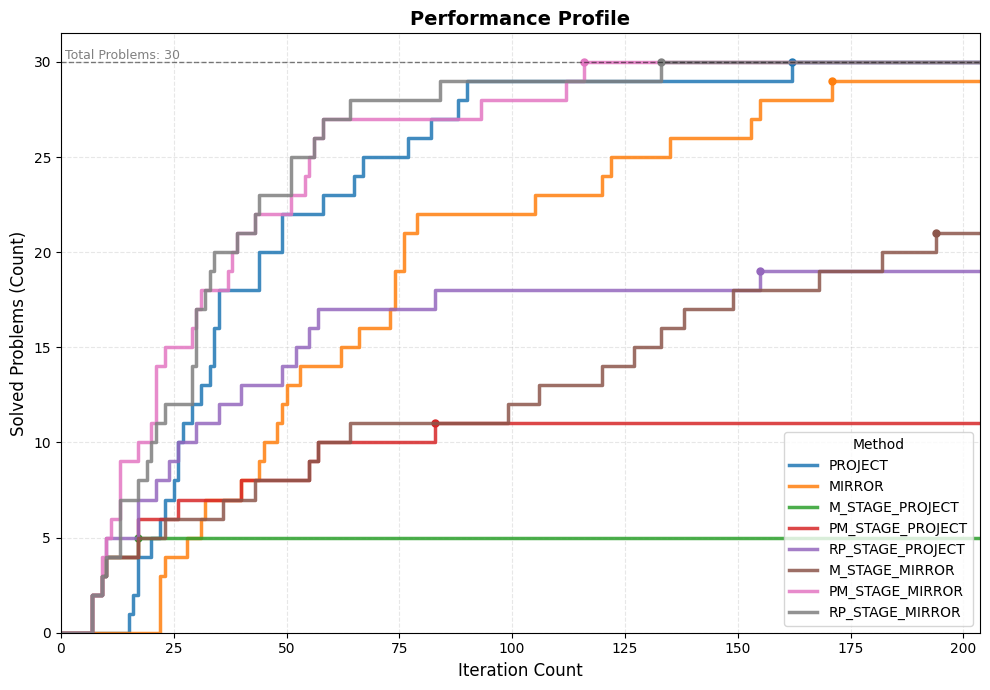
\includegraphics[width=0.75\textwidth]{results/iteration_performance_profile_2.png}
        \caption{Performance profile for different regularization techniques}
    \end{figure}
\end{frame}

\begin{frame}{Numerical experiments}
    \framesubtitle{Numerical results, Regularization counts}
        \begin{figure}[H]
        \centering
        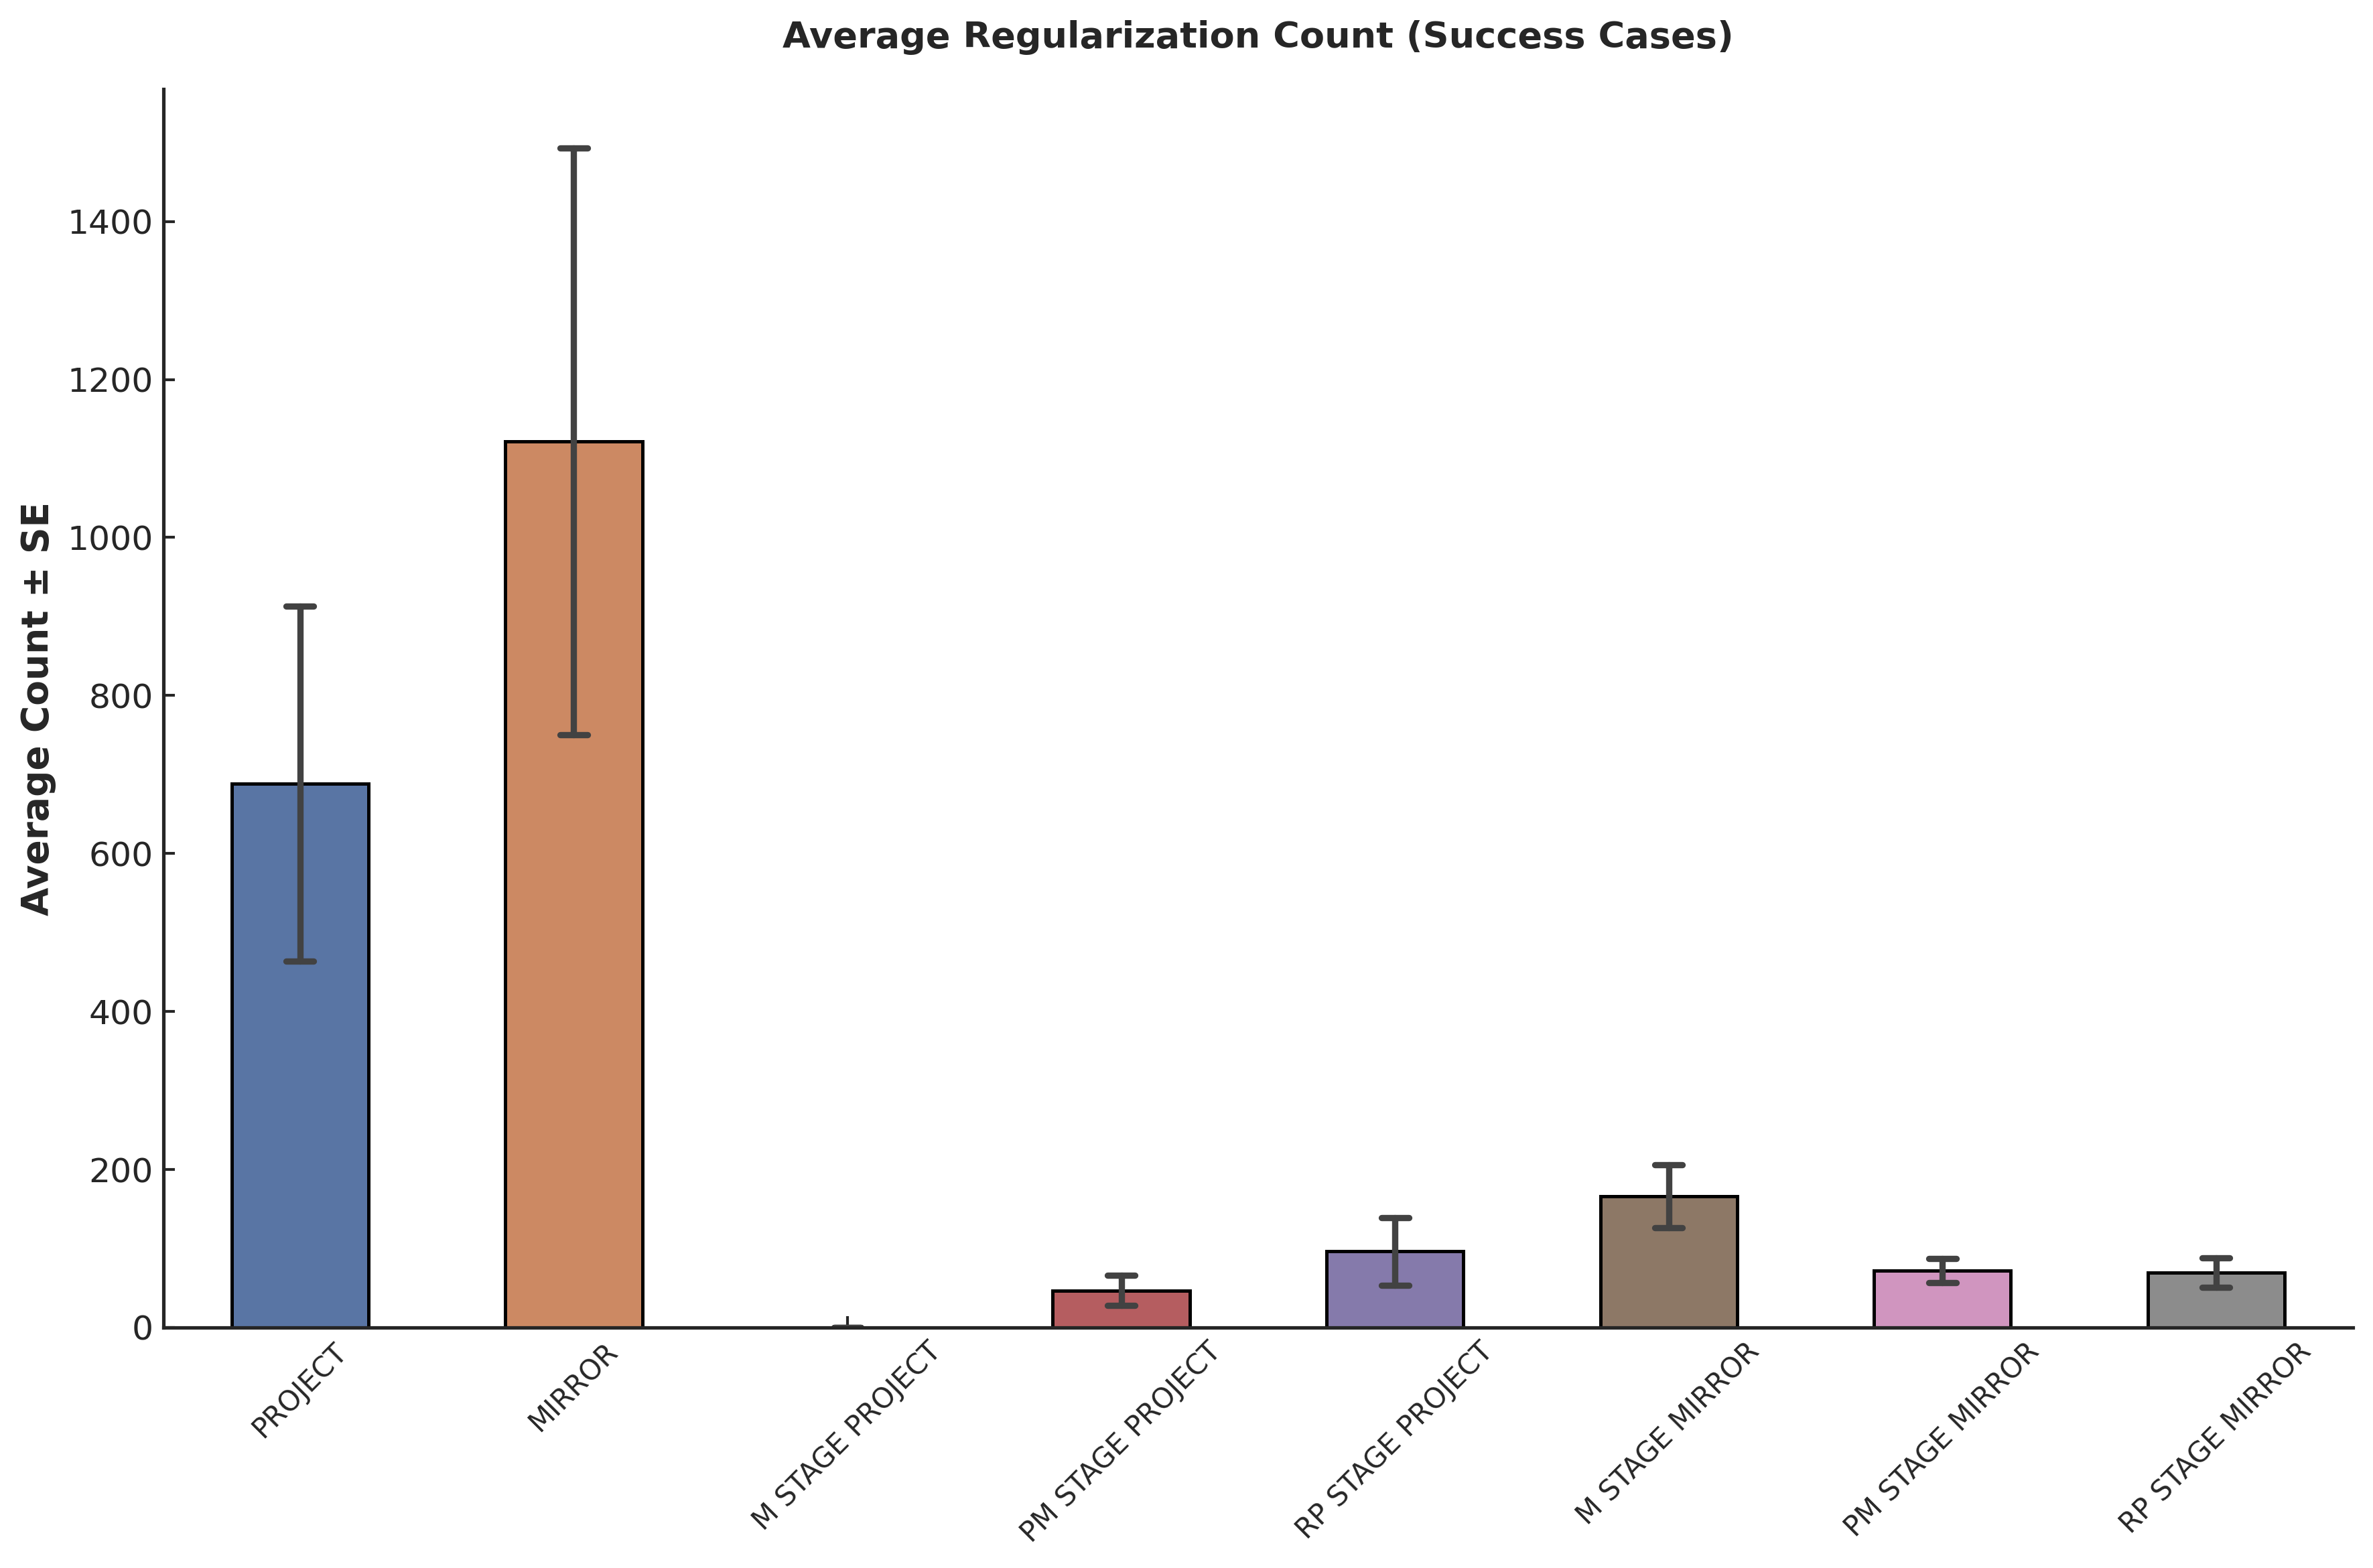
\includegraphics[width=0.75\textwidth]{results/regularization_avg_se.png}
        \caption{Average regularization counts per case for different regularization techniques}
    \end{figure}
\end{frame}


\begin{frame}{Numerical experiments}
    \framesubtitle{Numerical results, M Positive}
\begin{table}
        \centering
        \caption{Numerical Comparison of Regularization Techniques with $x_0 = [5.0, 5.0, 5.0]$}
        \setlength{\tabcolsep}{3pt}
        \begin{tabular}{c ccc ccc}
            \toprule
            % Using multirow to span the header height
            \multirow{2}{*}{\diagbox[width=6.5em, height=2.8em]{\textbf{Reg.}}{\textbf{Problem}}} &
            \multicolumn{3}{c}{M\_pos-R\_inde-P\_pos} & \multicolumn{3}{c}{M\_pos-R\_pos-P\_inde}\\
            % 3. \cmidrule(lr) creates gaps between groups, improving scannability
            \cmidrule(lr){2-4} \cmidrule(lr){5-7}
            & iter. & res. & stat. & iter. & res. & stat. \\
            \midrule
            NO\_REG.    	& 9 & 5.64e-10 & 0 	    & 18 & 1.78e-10 & 0 \\
            PROJECT     	& 63 & 9.83e-10 & 0 	& 24 & 6.59e-10 & 0 \\
            MIRROR      	& 116 & 8.69e-10 & 0 	& 33 & 4.77e-10 & 0 \\
            M\_STAGE\_P/M  	& 9 & 5.64e-10 & 0 	    & 18 & 1.78e-10 & 0 \\
            PM\_STAGE\_P/M  & 9 & 5.64e-10 & 0 	    & 18 & 1.78e-10 & 0 \\
            RP\_STAGE\_P/M  & 9 & 5.64e-10 & 0 	    & 18 & 1.78e-10 & 0 \\
            \bottomrule
        \end{tabular}
    \end{table}
    When M is Positive Definite, Full Hessian regularization leads to more iterations.
\end{frame}

\begin{frame}{Numerical experiments}
    \framesubtitle{Numerical results, M Indefinite}
    For the cases where M is Indefinite, we focus on the Reduced-hessian based methods and care about the following statistics:
    \begin{itemize}
        \item Max eigenvalue adjustment on M/P: Worst case for adjusting eigenvalue of M/P during regularization
        \item Max condition number reduction on M/P: The maximum decrease in the condition number of M/P during regularization
    \end{itemize}
\end{frame}

\begin{frame}{Numerical experiments}
    \framesubtitle{Numerical results, M Indefinite: Max eigenvalue adjustment}
    \begin{figure}
        \centering
        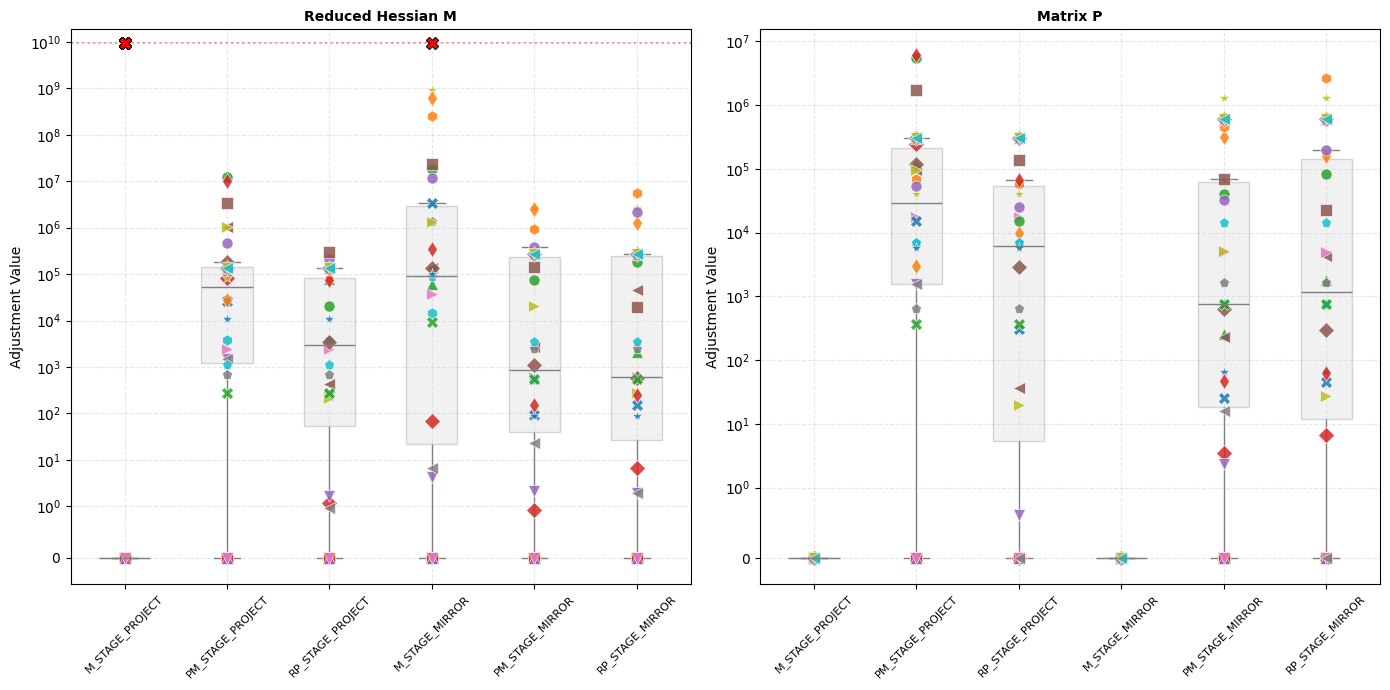
\includegraphics[width=1.0\textwidth]{results/adjustment.png}
        \caption{Max eigenvalue adjustment of M\&P for different regularization techniques}
    \end{figure}
\end{frame}

\begin{frame}{Numerical experiments}
    \framesubtitle{Numerical results, M Indefinite: Max condition number reduction}
    \begin{figure}
        \centering
        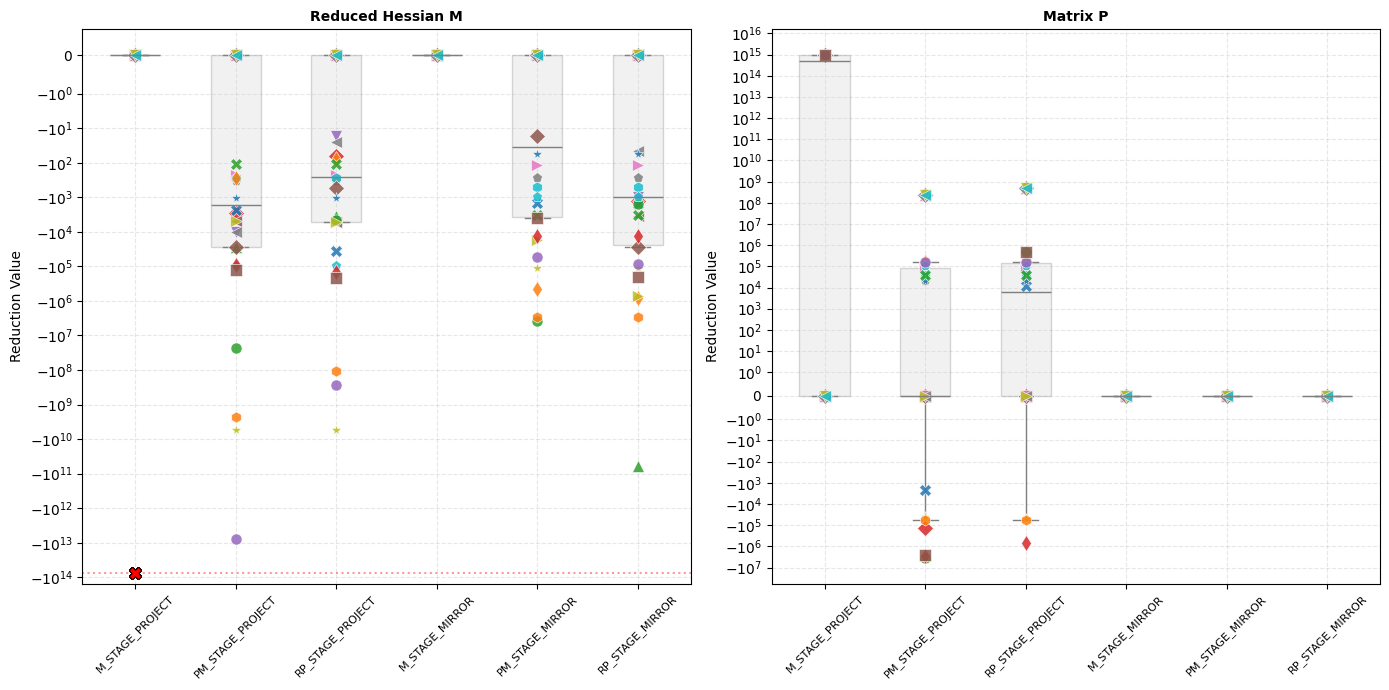
\includegraphics[width=1.0\textwidth]{results/reduction.png}
        \caption{Max condition number reduction of M\&P for different regularization techniques}
    \end{figure}
\end{frame}

\begin{frame}{Conclusion}
    \framesubtitle{Conclusion}
    \begin{itemize}
        \item Full Hessian vs Reduced Hessian
        \begin{itemize}
            \item Full Hessian regularization may lead to over-regularization when M is already positive definite
            \item Reduced Hessian regularization can avoid this based on recursion
        \end{itemize}
        \pause
        \item Regularization on P
        \begin{itemize}
            \item Regularizing P in Reduced Hessian regularization can help a lot in general
        \end{itemize}
        \pause
        \item PROJECT vs MIRROR
        \begin{itemize}
            \item PROJECT usually works better than MIRROR when regularizing full Hessian
            \item When it comes to Reduced Hessian regularization, MIRROR works better than PROJECT due to controlled condition number
        \end{itemize}
    \end{itemize}
\end{frame}

\begin{frame}{Thank you!}
    \begin{center}
        \Huge Thank you! \\
        \vspace{1em}
        \Large Questions?
    \end{center}
\end{frame}

\bibliographystyle{plain}

\end{document}
